\chapter{Research Framework\label{cha:method}}

\section{Objectives}

To achieve the research aim a number of objectives are proposed:
\begin{itemize}
  \item To determine student and institutional requirements for a lifelong learning
environment within the university context;
  \item To map these requirements against the e-tools, and ePortfolio system in
particular, already used in universities to support lifelong learning;
  \item To implement the features required in ePortfolio systems in conjunction
with LMS to satisfy the defined requirements;
  \item To evaluate how these combined systems meet the needs of all
stakeholders in supporting lifelong learning.
\end{itemize}

\section{Research Questions}

\begin{enumerate}
  \item \textit{What is the concept of \LLLs and its connection to the
  universities?}
	\begin{itemize}
	  \item What is the role of \LLLs in the university context?
	  \item What is the motivation of universities in supporting \LLLsn?
  	  \item What are the existing university policies for supporting \LLLsn?
      \item What are the components of \LLLs environments in universities?
      \item What are the requirements for successful \LLLs support in
   universities?
	\end{itemize} 
	
   \item \textit{What e-tools are available to support \LLLs within the
   university context?}
	\begin{itemize}
		\item What e-tools are available to support \LLLsn:
			\begin{itemize}
				\item in general?
				\item in universities?
			\end{itemize}
		\item What are the conceptual strengths and weaknesses of these e-tools in
university context?
		\item What is the relationship between LMS and e-tools support for \LLLs in
university context?
	\end{itemize}

	\item \textit{How can LMS and/or ePortfolio systems be extended to support
	students in a university context in \LLLsn?}
	\begin{itemize}
		\item What features are available now in these systems?
		\item What are the students and institutional requirements for LMS and
		ePortfolio to support \LLLsn?
		\item How can these requirements be translated and implemented into new or
		improved features?
	\end{itemize}

	\item \textit{Do this extended environment meet the needs of the stakeholders
in university teaching and learning contexts?}
	\begin{itemize}
		\item How can lecturers use new features to provide students with their
guidance and help them to understand \LLLs skills?
		\item How can students address institutional graduate attributes and other
		skills using new features?
		\item How can new features help students track their learning progress, manage
ePortfolio knowledge and content, demonstrate and share their achievements
with others?
	\end{itemize}
\end{enumerate}

\section{Research Approach}

\subsection{Design Science Research Methodology}

\subsection{Design Science Research Applied to This Project}

\subsubsection{Stage 1. Problem identification and motivation}

\subsubsection{Stage 2. Objectives for a Solution}

\subsubsection{Stage 3. Design and Development}

The prototype development in this project followed established
software engineering practices that interleaved coding and revision, forming
iterative development cycles, as it shown at ~\ref{fig:prototype}.

\begin{figure}[htb]
\centering
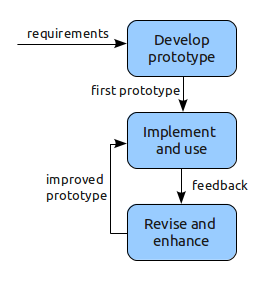
\includegraphics[height=0.3\textheight]{CH2-F2-Prototype}
\caption[Ptototyping]{Prototyping (based on \citet*[p.~411]{Sommerville2007})}
\label{fig:prototype}
\end{figure}

\subsubsection{Stage 4. Demonstration}

\subsubsection{Stage 5. Evaluation}

\subsubsection{Stage 6. Communication}

\section{Methodological Limitations}

\section{Summary}